%%% Preamble
\documentclass[paper=a4, fontsize=11pt]{scrartcl}


\usepackage{float}
%\usepackage{geometry} %AGREGOOOOO
%\geometry{verbose,tmargin=2cm,bmargin=2cm,lmargin=2cm,rmargin=2cm,headheight=2cm,headsep=2cm}
%\geometry{verbose,tmargin=2cm,bmargin=2cm,lmargin=2cm,rmargin=2cm,headheight=2cm,headsep=2cm}
\usepackage{multirow}



\usepackage[T1]{fontenc}
\usepackage{fourier}
\usepackage[utf8]{inputenc}
\usepackage[english]{babel}					% English language/hyphenation

\usepackage[protrusion=true,expansion=true]{microtype}	
\usepackage{amsmath,amsfonts,amsthm} % Math packages
\usepackage[pdftex]{graphicx}	
\usepackage{url} %SACO ESTO
\usepackage{import}

\usepackage[margin=2cm]{geometry}
\geometry{verbose,tmargin=2cm,bmargin=2cm,lmargin=2cm,rmargin=2cm,headheight=2cm,headsep=2cm} %SACO ESTO
% %%% Custom sectioning
\usepackage{sectsty}
\allsectionsfont{\normalfont \scshape}


%%COMENTO ESTO

%%% Custom headers/footers (fancyhdr package)
%\usepackage{fancyhdr}
%\pagestyle{fancyplain}
%\fancyhead{}											% No page header
%\fancyfoot[L]{}											% Empty 
%\fancyfoot[C]{}											% Empty
%\fancyfoot[R]{\thepage}									% Pagenumbering
%\renewcommand{\headrulewidth}{0pt}			% Remove header underlines
%\renewcommand{\footrulewidth}{0pt}				% Remove footer underlines
%\setlength{\headheight}{13.6pt}




%%% Equation and float numbering
\numberwithin{equation}{section}		% Equationnumbering: section.eq#
\numberwithin{figure}{section}			% Figurenumbering: section.fig#
\numberwithin{table}{section}				% Tablenumbering: section.tab#


%%% Maketitle metadata
\newcommand{\horrule}[1]{\rule{\linewidth}{#1}} 	% Horizontal rule

%AGREGO PARA EJ 1
\usepackage{graphicx}
\usepackage{color} 
\usepackage[dvipsnames]{xcolor}
\colorlet{purple}{purple}

%/////////////////////////////////// AGREGO PARA EL EJ 2

    \usepackage{geometry} % Required to change the page size to A4
    \geometry{a4paper} % Set the page size to be A4 as opposed to the default US Letter

    \usepackage{mathtools, nccmath}
     
    
    
%%%%%%%%%%%%% AGREGOOOOO
\usepackage{xcolor}



    \usepackage{tikz}
    \usetikzlibrary{matrix,calc}

    %isolated term
%#1 - Optional. Space between node and grouping line. Default=0
%#2 - node
%#3 - filling color
\newcommand{\implicantsol}[3][0]{
    \draw[rounded corners=3pt, fill=#3, opacity=0.3] ($(#2.north west)+(135:#1)$) rectangle ($(#2.south east)+(-45:#1)$);
    }


%internal group
%#1 - Optional. Space between node and grouping line. Default=0
%#2 - top left node
%#3 - bottom right node
%#4 - filling color
\newcommand{\implicant}[4][0]{
    \draw[rounded corners=3pt, fill=#4, opacity=0.3] ($(#2.north west)+(135:#1)$) rectangle ($(#3.south east)+(-45:#1)$);
    }

%group lateral borders
%#1 - Optional. Space between node and grouping line. Default=0
%#2 - top left node
%#3 - bottom right node
%#4 - filling color
\newcommand{\implicantcostats}[4][0]{
    \draw[rounded corners=3pt, fill=#4, opacity=0.3] ($(rf.east |- #2.north)+(90:#1)$)-| ($(#2.east)+(0:#1)$) |- ($(rf.east |- #3.south)+(-90:#1)$);
    \draw[rounded corners=3pt, fill=#4, opacity=0.3] ($(cf.west |- #2.north)+(90:#1)$) -| ($(#3.west)+(180:#1)$) |- ($(cf.west |- #3.south)+(-90:#1)$);
}

%group top-bottom borders
%#1 - Optional. Space between node and grouping line. Default=0
%#2 - top left node
%#3 - bottom right node
%#4 - filling color
\newcommand{\implicantdaltbaix}[4][0]{
    \draw[rounded corners=3pt, fill=#4, opacity=0.3] ($(cf.south -| #2.west)+(180:#1)$) |- ($(#2.south)+(-90:#1)$) -| ($(cf.south -| #3.east)+(0:#1)$);
    \draw[rounded corners=3pt, fill=#4, opacity=0.3] ($(rf.north -| #2.west)+(180:#1)$) |- ($(#3.north)+(90:#1)$) -| ($(rf.north -| #3.east)+(0:#1)$);
}

%group corners
%#1 - Optional. Space between node and grouping line. Default=0
%#2 - filling color
\newcommand{\implicantcantons}[2][0]{
    \draw[rounded corners=3pt, opacity=.3] ($(rf.east |- 0.south)+(-90:#1)$) -| ($(0.east |- cf.south)+(0:#1)$);
    \draw[rounded corners=3pt, opacity=.3] ($(rf.east |- 8.north)+(90:#1)$) -| ($(8.east |- rf.north)+(0:#1)$);
    \draw[rounded corners=3pt, opacity=.3] ($(cf.west |- 2.south)+(-90:#1)$) -| ($(2.west |- cf.south)+(180:#1)$);
    \draw[rounded corners=3pt, opacity=.3] ($(cf.west |- 10.north)+(90:#1)$) -| ($(10.west |- rf.north)+(180:#1)$);
    \fill[rounded corners=3pt, fill=#2, opacity=.3] ($(rf.east |- 0.south)+(-90:#1)$) -|  ($(0.east |- cf.south)+(0:#1)$) [sharp corners] ($(rf.east |- 0.south)+(-90:#1)$) |-  ($(0.east |- cf.south)+(0:#1)$) ;
    \fill[rounded corners=3pt, fill=#2, opacity=.3] ($(rf.east |- 8.north)+(90:#1)$) -| ($(8.east |- rf.north)+(0:#1)$) [sharp corners] ($(rf.east |- 8.north)+(90:#1)$) |- ($(8.east |- rf.north)+(0:#1)$) ;
    \fill[rounded corners=3pt, fill=#2, opacity=.3] ($(cf.west |- 2.south)+(-90:#1)$) -| ($(2.west |- cf.south)+(180:#1)$) [sharp corners]($(cf.west |- 2.south)+(-90:#1)$) |- ($(2.west |- cf.south)+(180:#1)$) ;
    \fill[rounded corners=3pt, fill=#2, opacity=.3] ($(cf.west |- 10.north)+(90:#1)$) -| ($(10.west |- rf.north)+(180:#1)$) [sharp corners] ($(cf.west |- 10.north)+(90:#1)$) |- ($(10.west |- rf.north)+(180:#1)$) ;
}

%Empty Karnaugh map 4x4
\newenvironment{Karnaugh}%
{
\begin{tikzpicture}[baseline=(current bounding box.north),scale=0.8]
\draw (0,0) grid (4,4);
\draw (0,4) -- node [pos=0.7,above right,anchor=south west] {y2 y1} node [pos=0.75,below left,anchor=north east] {w y3} ++(135:1);
%
\matrix (mapa) [matrix of nodes,
        column sep={0.8cm,between origins},
        row sep={0.8cm,between origins},
        every node/.style={minimum size=0.3mm},
        anchor=8.center,
        ampersand replacement=\&] at (0.5,0.5)
{
                       \& |(c00)| 00         \& |(c01)| 01         \& |(c11)| 11         \& |(c10)| 10         \& |(cf)| \phantom{00} \\
|(r00)| 00             \& |(0)|  \phantom{0} \& |(1)|  \phantom{0} \& |(3)|  \phantom{0} \& |(2)|  \phantom{0} \&                     \\
|(r01)| 01             \& |(4)|  \phantom{0} \& |(5)|  \phantom{0} \& |(7)|  \phantom{0} \& |(6)|  \phantom{0} \&                     \\
|(r11)| 11             \& |(12)| \phantom{0} \& |(13)| \phantom{0} \& |(15)| \phantom{0} \& |(14)| \phantom{0} \&                     \\
|(r10)| 10             \& |(8)|  \phantom{0} \& |(9)|  \phantom{0} \& |(11)| \phantom{0} \& |(10)| \phantom{0} \&                     \\
|(rf) | \phantom{00}   \&                    \&                    \&                    \&                    \&                     \\
};
}%
{
\end{tikzpicture}
}

%Empty Karnaugh map 2x4
\newenvironment{Karnaughvuit}%
{
\begin{tikzpicture}[baseline=(current bounding box.north),scale=0.8]
\draw (0,0) grid (4,2);
\draw (0,2) -- node [pos=0.7,above right,anchor=south west] {y2 y1} node [pos=0.7,below left,anchor=north east] {y3} ++(135:1);
%
\matrix (mapa) [matrix of nodes,
        column sep={0.8cm,between origins},
        row sep={0.8cm,between origins},
        every node/.style={minimum size=0.3mm},
        anchor=4.center,
        ampersand replacement=\&] at (0.5,0.5)
{
                      \& |(c00)| 00         \& |(c01)| 01         \& |(c11)| 11         \& |(c10)| 10         \& |(cf)| \phantom{00} \\
|(r00)| 0             \& |(0)|  \phantom{0} \& |(1)|  \phantom{0} \& |(3)|  \phantom{0} \& |(2)|  \phantom{0} \&                     \\
|(r01)| 1             \& |(4)|  \phantom{0} \& |(5)|  \phantom{0} \& |(7)|  \phantom{0} \& |(6)|  \phantom{0} \&                     \\
|(rf) | \phantom{00}  \&                    \&                    \&                    \&                    \&                     \\
};
}%
{
\end{tikzpicture}
}

%Empty Karnaugh map 2x2
\newenvironment{Karnaughquatre}%
{
\begin{tikzpicture}[baseline=(current bounding box.north),scale=0.8]
\draw (0,0) grid (2,2);
\draw (0,2) -- node [pos=0.7,above right,anchor=south west] {b} node [pos=0.7,below left,anchor=north east] {a} ++(135:1);
%
\matrix (mapa) [matrix of nodes,
        column sep={0.8cm,between origins},
        row sep={0.8cm,between origins},
        every node/.style={minimum size=0.3mm},
        anchor=2.center,
        ampersand replacement=\&] at (0.5,0.5)
{
          \& |(c00)| 0          \& |(c01)| 1  \\
|(r00)| 0 \& |(0)|  \phantom{0} \& |(1)|  \phantom{0} \\
|(r01)| 1 \& |(2)|  \phantom{0} \& |(3)|  \phantom{0} \\
};
}%
{
\end{tikzpicture}
}

%Defines 8 or 16 values (0,1,X)
\newcommand{\contingut}[1]{%
\foreach \x [count=\xi from 0]  in {#1}
     \path (\xi) node {\x};
}

%Places 1 in listed positions
\newcommand{\minterms}[1]{%
    \foreach \x in {#1}
        \path (\x) node {1};
}

%Places 0 in listed positions
\newcommand{\maxterms}[1]{%
    \foreach \x in {#1}
        \path (\x) node {0};
}

%Places X in listed positions
\newcommand{\indeterminats}[1]{%
    \foreach \x in {#1}
        \path (\x) node {X};
}

    \linespread{1.2} % Line spacing
    
    \setlength\parindent{0pt} % Uncomment to remove all indentation from paragraphs
    
   % \graphicspath{{/home/bzerol/VisualCode/ElectroIII/tp1-team-2/E2TP1}} % Specifies the directory where pictures are stored

%//////////////////////////////////// agrego para EJ 4
%\documentclass[english]{article}
%\usepackage[T1]{fontenc}
%\usepackage[latin9]{inputenc}
%\usepackage{geometry}
%\geometry{verbose,tmargin=2cm,bmargin=2cm,lmargin=2cm,rmargin=2cm,headheight=2cm,headsep=2cm}
%\usepackage{float}
%\usepackage{graphicx}

\makeatletter

%%%%%%%%%%%%%%%%%%%%%%%%%%%%%% LyX specific LaTeX commands.
%% Because html converters don't know tabularnewline
\providecommand{\tabularnewline}{\\}

%%%%%%%%%%%%%%%%%%%%%%%%%%%%%% User specified LaTeX commands.
\usepackage{babel}


\makeatother

\usepackage{babel}

%///////////////////////////// PARA EL EJ6
%\documentclass[english]{article}
%\usepackage[T1]{fontenc}
%\usepackage[latin9]{inputenc}
%\usepackage{geometry}
%\geometry{verbose,tmargin=3cm,bmargin=3cm,lmargin=3cm,rmargin=3cm,headheight=3cm,headsep=3cm}
%\usepackage{float}

%\makeatletter

%%%%%%%%%%%%%%%%%%%%%%%%%%%%%% LyX specific LaTeX commands.
%% Because html converters don't know tabularnewline
\providecommand{\tabularnewline}{\\}



%%AGREG0 
\usepackage{tikz}
\usetikzlibrary{shapes,arrows}

\tikzstyle{decision} = [diamond, draw, fill=blue!20, 
    text width=4.5em, text badly centered, node distance=4cm, inner sep=0pt]
\tikzstyle{block} = [rectangle, draw, fill=blue!20, 
    text width=5em, text centered, rounded corners, minimum height=2em]
\tikzstyle{line} = [draw, -latex']
\tikzstyle{cloud} = [draw, ellipse,fill=red!20, node distance=3cm,
    minimum height=2em]

\usepackage{listings}

\usepackage[utf8]{inputenc}
 
\usepackage{listings}
%\usepackage{color}
 
\definecolor{codegreen}{rgb}{0,0.6,0}
\definecolor{codegray}{rgb}{0.5,0.5,0.5}
\definecolor{codepurple}{rgb}{0.58,0,0.82}
\definecolor{backcolour}{rgb}{0.95,0.95,0.92}
 
\lstdefinestyle{mystyle}{
    backgroundcolor=\color{backcolour},   
    commentstyle=\color{codegreen},
    keywordstyle=\color{magenta},
    numberstyle=\tiny\color{codegray},
    stringstyle=\color{codepurple},
    basicstyle=\footnotesize,
    breakatwhitespace=false,         
    breaklines=true,                 
    captionpos=b,                    
    keepspaces=true,                 
    numbers=left,                    
    numbersep=5pt,                  
    showspaces=false,                
    showstringspaces=false,
    showtabs=false,                  
    tabsize=2
}
 
\lstset{style=mystyle}


\usepackage[utf8]{inputenc}

%\DeclareUnicodeCharacter{00A0}{ }

%\DeclareUnicodeCharacter{00A0}{~}
%\newunicodechar{^^a0}{~}

\begin{document}

\title{
	\usefont{OT1}{bch}{b}{n}
	\normalfont \normalsize \textsc{Instituto Tecnológico de Buenos Aires} \\ [25pt]
	\horrule{2pt} \\[0.4cm]
	\huge Trabajo Pr\'actico 2\\
	\horrule{2pt} \\[0cm]
\author{Grupo 2:\\M\'aspero, Martina \\Mestanza, Joaqu\'in\\ Müller, Malena\\Nowik, Ariel\\Regueira, Marcelo\\ \\ }
\text{Señales Aleatorias - 2019}
}
\date{\today} 
\pagenumbering{arabic}

\maketitle
\newpage

%%%%%%%%%%%%%%%%%%%%%%%%%%%%%
\section*{Ejercicio 1}

En esta parte del trabajo se estiman algunos par\'ametros de la secuencia aleatoria X(n) del archivo que se nos ha sido enviado.

%%
\subsection{Estimaci\'on de los primeros 128 valores de la funci\'on de autocorrelaci\'on utilizando los estimadores no polarizado y polarizado}

El estimador no polarizado de la autocorrelación está dado por la expresión (de la página 567 del libro ``Random Signals'', K. Sam Shanmugan):
$$R_{xx_{np}}(k) = \frac{1}{N - k} \sum_{i=1}^{N-k-1}X(i)X(i+k)$$
Donde $N$ es la cantidad de muestras asignadas, que en este caso son 4096. Los valores que toma $k$ son entre 0 y 127, para obtener los 128 primeros valores solicitados.\par

El estimador polarizado esta dado por la expresión (de la página 571 del libro):

$$R_{xx_{p}}(k) = \frac{1}{N} \sum_{i=1}^{N-k-1}X(i)X(i+k)$$
Para los mismos valores de $k$ y $N$ previamente mencionados.

Al normalizar con $R_{xx_{NP}}(0)$ cada uno de los valores estimados de esta manera,  se obtienen los coeficientes de autocorrelación total $r_{xx_{NP}}(k)$ (no polarizado) y $r_{xx_{P}}$ (polarizado), que se pueden ver graficados en las figuras \ref{rxxNP} y \ref{rxxP}, respectivamente.

El c\'odigo implementado para realizar esto, es el siguiente:

%%%%%%
\begin{lstlisting}[language=Matlab, caption=EJ1.m]
%% ITEM 1
clear all;
clc;

S = load('Archivo_2.mat');
%whos S
%whos -file Archivo_2.mat

N = 4096;
length = 128;
% Estimador no polarizado y polarizado
RxxNP = zeros(length, 1); %contendr\'a el RxxNP para cada valor de k entre 0 y 127
RxxP = zeros(length, 1); %contendr\'a el RxxP para cada valor de k entre 0 y 127
for k = 0:length-1
    sum = 0;
    for i = 0:N-k-1
        sum = sum + (S.x(i+1) * S.x(i+1+k));
    end
    RxxNP(k+1) = (1/(N-k)) * sum;
    RxxP(k+1) = (1/N) * sum; 
end

clearvars sum;
clearvars i;
clearvars k;

% Coeficiente de correlacion
rxxNP = RxxNP/RxxNP(1);
rxxP = RxxP/RxxP(1);

k = 0:1:length-1;
figure;
plot(k,rxxNP)
figure;
plot(k,rxxP)
\end{lstlisting}

\begin{figure}[H] %!ht
\centering
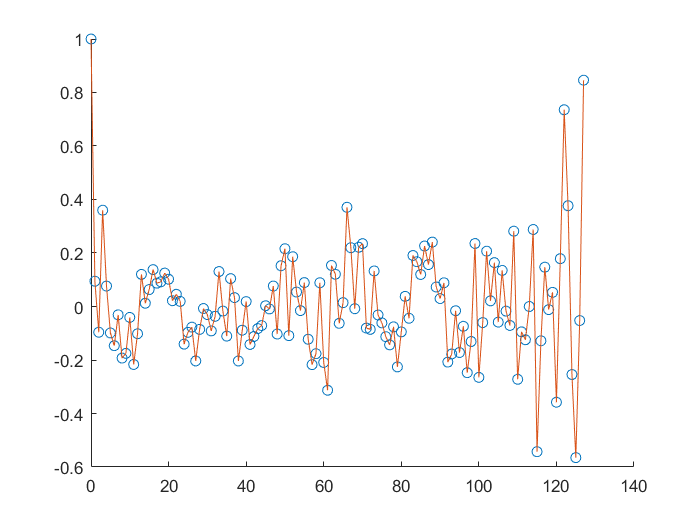
\includegraphics[scale=0.45]{../EJ1/rxxNP}
\caption{$r_{xx}(k)$ a partir del estimador no polarizado.}
\label{rxxNP}
\end{figure}

\begin{figure}[H] %!ht
\centering
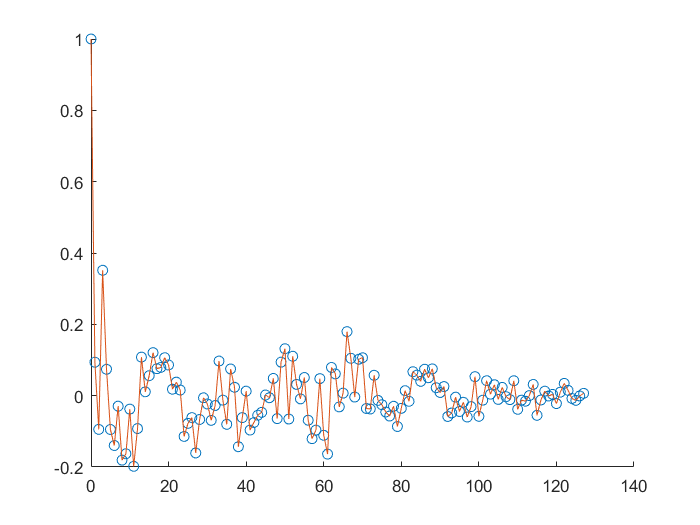
\includegraphics[scale=0.45]{../EJ1/rxxP}
\caption{$r_{xx}(k)$ a partir del estimador polarizado.}
\label{rxxP}
\end{figure}

En una primera instancia, se superpuso las dos gráficas para poder denotar diferencias, pero resultaron ser casi iguales. Esto se deriva de que un estimador se encuentra dividido por $N$, y el otro por $N-k$. Siendo 127 el mayor valor que puede tomar $k$, sigue siendo pequeño en comparación a $N$, que es 4096, por lo que no afecta significativamente a los resultados. 

\newpage

\subsection{Estimaci\'on de los primeros 128 coeficientes de correlaci\'on parcial}

Para calcular los coeficientes de correlación parcial $\phi_{k,k}$, se arma la matriz de toeplitz correspondiente para cada $k$, y con ella se resuelve la ecuación de Yule-Walker (de la página 262 del libro):

\[
r_{xx} = R \cdot \Phi
\]

Donde $R$ es la matriz de coeficientes de autocorrelación (que es una matriz de toeplitz) y $\Phi$ el vector de coeficientes $\phi_{p,k}$. De dicho vector, se utiliza solamente el último elemento (donde $p=k$) en cada caso, y se lo almacena en otro vector nuevo para tener todos los coeficientes de correlación parcial. Se graficaron los coeficientes obtenidos tanto para el caso no polarizado como para el polarizado. También resultaron ambos casos valores muy similares, por lo que se separaron las gráficas al igual que antes.

A continuaci\'on se presenta el c\'odigo:

\begin{lstlisting}[language=Matlab, caption=EJ1.m]
%% ITEM 2
length = 127;

%Caso a partir de estimacion de Rxx NO polarizado
partialCorrCoefNP = zeros (1, length) %contendr\'a los coeficientes de 
                                  %correlaci\'on parcial para k entre 1 y 127
                                  %a partir del caso no polarizado.

rxxNPaux = rxxNP                               
for k = 1:length
    rxxToep = toeplitz(rxxNPaux') % Se genera la matriz de Toeplitz
    rxxMat = rxxToep(1:k,1:k)
    rxxVect = (rxxNPaux(2:k+1));
    corrCoefVect = inv(rxxMat) * rxxVect; % Se resuelve la ecuacion de Yule Walker
    partialCorrCoefNP(k)= corrCoefVect(k);
end

%Caso a partir de estimacion de Rxx polarizado
partialCorrCoefP = zeros(1,length); % contendra los coeficientes de 
                                 %correlacion parcial para k entre 1 y 127; 
                                 %a partir del caso polarizado
rxxPaux = rxxP;                                
for k = 1:length
    rxxToep = toeplitz(rxxPaux'); % Generating Toeplitz Matrix
    rxxMat = rxxToep(1:k,1:k);
    rxxVect = (rxxPaux(2:k+1));
    corrCoefVect = inv(rxxMat) * rxxVect; % Solving Yule Walker Equation
    partialCorrCoefP(k)= corrCoefVect(k);
end
q = 1:length;
figure
stem(q,partialCorrCoefNP)

q = 1:length;
figure
stem(q,partialCorrCoefP)
\end{lstlisting}

\begin{figure}[H] %!ht
\centering
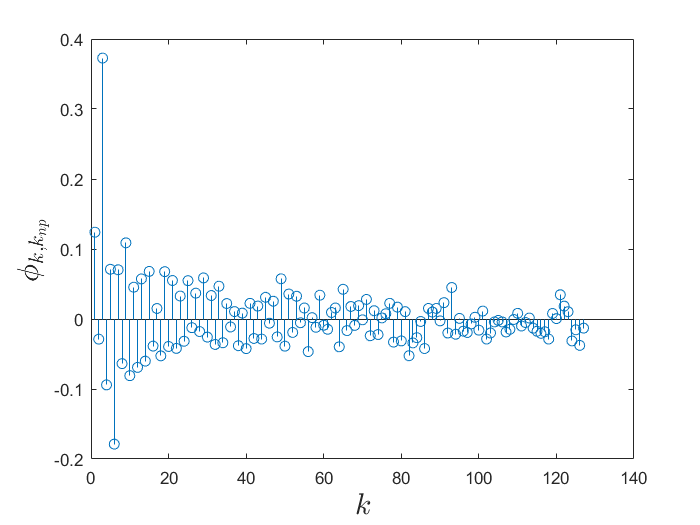
\includegraphics[scale=0.45]{../EJ1/coefCorrParcialNP}
\caption{Coeficientes de correlaci\'on parcial a partir del estimador no polarizado.}
\label{fiNP}
\end{figure}

\begin{figure}[H] %!ht
\centering
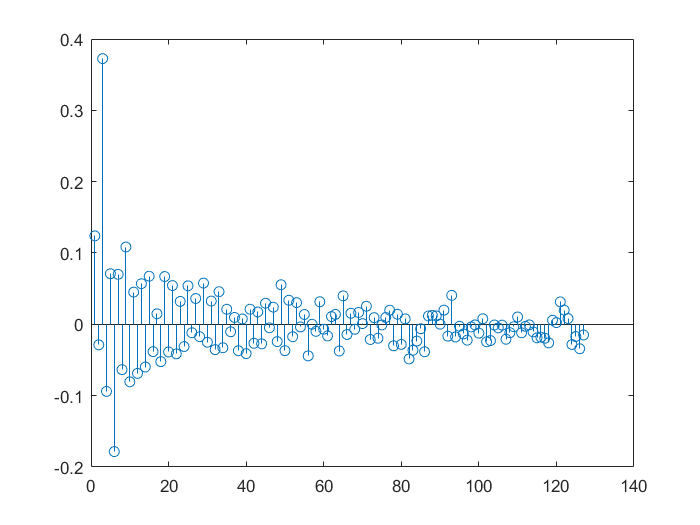
\includegraphics[scale=0.45]{../EJ1/coefCorrParcialP}
\caption{Coeficientes de correlaci\'on parcial a partir del estimador polarizado.}
\label{fiP}
\end{figure}

%%
\subsection{Determinaci\'on del modelo y orden para ajustar a la secuencia aleatoria $X(n)$}

Luego de probar con modelos AR, MA de segundo orden y ARMA(1,1), se determin\'o que el que mejor ajusta a la secuencia aleatoria $X(n)$ podr\'ia ser el AR de orden 2. Teniendo en cuenta que la entrada es una secuencia de ruido blanco y Gaussiano con varianza unitaria, se hallan los par\'ametros de este modelo. Se planteó solo el caso no polarizado, dado que se obtienen resultados muy similares como ocurrió previamente, por lo que se deja solo uno como caso representativo.\par
Del vector de los $R_{xx_{np}}(k)$ obtenidos, se toman el $R_{xx_{np}}(0) = 1.3690$, $R_{xx_{np}}(1) = 0.1698$ y $R_{xx_{np}}(2) = -0.0178$.\par A partir de la expresión recursiva para la autocorrelación de un modelo AR de orden 2 (de la página 257 del libro):

\[
R_{xx}(k) = \phi_{2,1} \cdot R_{xx}(k-1) + \phi_{2,2} \cdot R_{xx}(k-2)
\]

Teniendo además en cuenta que $R_{xx}(k) = R_{xx}(-k)$, se plantean dos ecuaciones:

\[
\left\{
\begin{array}{lll}
     \phi_{2,1} \cdot R_{xx}(0) + \phi_{2,2} \cdot R_{xx}(1) & = & R_{xx}(1) 
  \\ \phi_{2,1} \cdot R_{xx}(1) + \phi_{2,2} \cdot R_{xx}(0) & = & R_{xx}(2)
\end{array}
\right.
\]

De donde se obtiene que $\phi_{2,1} = 0.1276$ y $\phi_{2,2} = -0.0288$. Con dichos valores, se calcula anal\'iticamente $R_{xx}(k)$ con la fórmula recursiva previamente planteada y $ r_{xx}(k) $, con $k$ entero entre 0 y 127. 

El código empleado es el siguiente:

\begin{lstlisting}[language=Matlab, caption=EJ1.m]
%% ITEM 3
% El AR(2) aparentemente lo describe
% X(n) = phi21*X(n-1) + phi22*X(n-2) + e(n)
phi21 = 0.1276;
phi22 = -0.0288;

%% ITEM 4

Rxx_TNP = zeros(length,1);
Rxx_TNP(1) = RxxNP(1);
Rxx_TNP(2) = RxxNP(2);

for k = 3:length-1
   Rxx_TNP(k) = phi21.*Rxx_TNP(k-1) + phi22.*Rxx_TNP(k-2); 
end
rxx_TNP = Rxx_TNP/Rxx_TNP(1);

k = 0:1:length-1;
figure
plot(k,rxx_TNP)

Rxx_TP = zeros(length,1);
Rxx_TP(1) = RxxP(1);
Rxx_TP(2) = RxxP(2);

for k = 3:length-1
   Rxx_TP(k) = phi21.*Rxx_TP(k-1) + phi22.*Rxx_TP(k-2); 
end
rxx_TP = Rxx_TP/Rxx_TP(1);

k = 0:1:length-1;
figure
plot(k,rxx_TP)
\end{lstlisting}
%%%%%%%

La gráfica obtenida se muestra a continuación.

\begin{figure}[H] %!ht
\centering
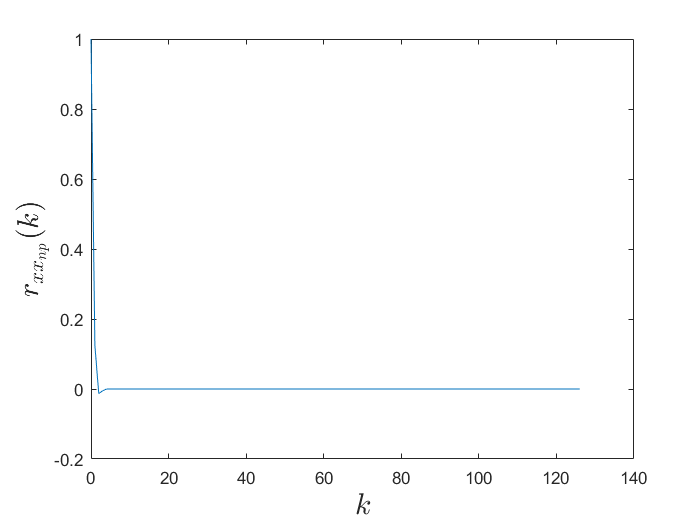
\includegraphics[scale=0.45]{../EJ1/rxxNPteorico}
\caption{$r_{xx}(k)$ a partir del estimador no polarizado, obtenido en forma teórica, en base al modelo AR orden 2.}
\label{rxxTeo}
\end{figure}

La curva obtenida se asemeja a la estimada con los valores al principio, y luego se anula prácticamente. Esto es consistente con el rápido decaimiento que posee la curva hallada en la figura \ref{rxxNP}, donde los valores más allá de $k=10$ se observó que se encuentran todos en el orden de $10^{-2}$.

\subsection{Estimaci\'on de la densidad espectral de potencia de X(n)}

En primer lugar, se estima la densidad espectral de potencia a partir de la transformada de Fourier discreta de la autocorrelación no polarizada. Por el mismo motivo mencionado anteriormente, se muestra solamente la resultante del caso no polarizado, dado que la otra es prácticamente similar. Los resultados pueden observarse en la figura \ref{densidadEs}. Se muestra también el código implementado para el cálculo de la transformada.

\begin{lstlisting}[language=Matlab, caption=EJ1.m]
%% ITEM 5
% Por transformada
SxxNP = fft(RxxNP);
mag_SxxNP = abs(SxxNP);
SxxNP(mag_SxxNP<1e-6) = 0;
f = 0:1:length;
figure
plot(f,mag_SxxNP)
\end{lstlisting}

\begin{figure}[H] %!ht
\centering
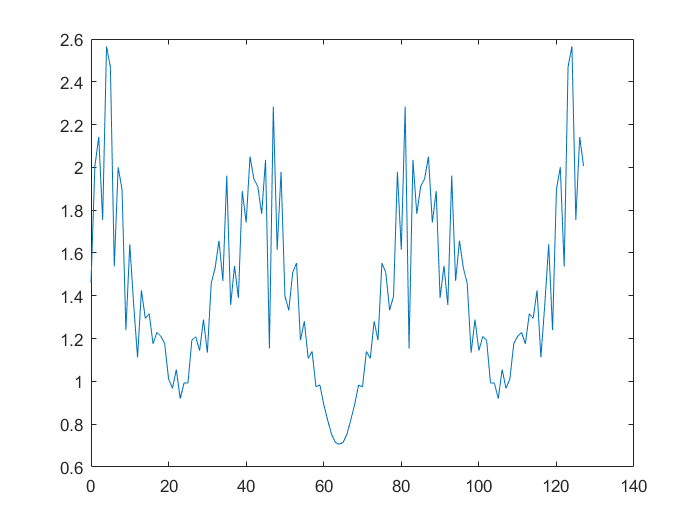
\includegraphics[scale=0.45]{../EJ1/densidadEspectralFourierDiscNP}
\caption{Estimaci\'on de la densidad espectral de potencia  de X(n) a partir de la transformada de Fourier discreta de la estimaci\'on de la autocorrelación no polarizada.}
\label{densidadEs}
\end{figure}

Por otro lado, se estima la densidad espectral de potencia a partir de la promediaci\'on de periodogramas. Para ello, las muestras iniciales se las divide en 16 grupos de 256 muestras cada uno. En cada grupo, se estiman los primeros 128 valores de la autocorrelación (no polarizado). A cada vector resultante, se le calcula la densidad espectral de potencia, y finalmente se las promedia (página 579 del libro): 

\[
\overline{S_{xx}}(f) = \frac{1}{n} \sum_{k=1}^n S_{xx}(f)_k
\]

Donde en este caso $n=16$. Pueden verse los resultados en la figura \ref{perio}. Se muestra también el código que implementa el procedimiento.

\begin{lstlisting}[language=Matlab, caption=EJ1.m]
% Por periodogramas
Rxx_Vector = zeros(16,128);
% Se divide la entrada en 16 grupos de 256 muestras, calculando
% a 16 funciones de autocorrelacion sus 128 primeros valores
% para el caso no polarizado
for l = 1:16
    for k = 0:127
        sum = 0;
        for i = 0:256-k-1
            sum = sum + (S.x(256*(l-1)+i+1) * S.x(256*(l-1)+i+1+k));
        end
        Rxx_Vector(l,k+1) = (1/(256-k)) * sum;
    end
end
Sxx_Vector = zeros(128,16);
% Se calcula la densidad espectral de cada uno
for k = 1:16
    Sxx_Vector(:,k) = fft(Rxx_Vector(k,:));
end
Sxx_Vector = Sxx_Vector';
Sxx_Med = zeros(1,128);
% Se estima la densidad promedio
for k = 1:16
    Sxx_Med = Sxx_Med + Sxx_Vector(k,:);
end
Sxx_Med = Sxx_Med/16;
mag_SxxMed = abs(Sxx_Med);
SxxNP(mag_SxxMed<1e-6) = 0;
figure
plot(1:128,mag_SxxMed)
\end{lstlisting}


\begin{figure}[H] %!ht
\centering
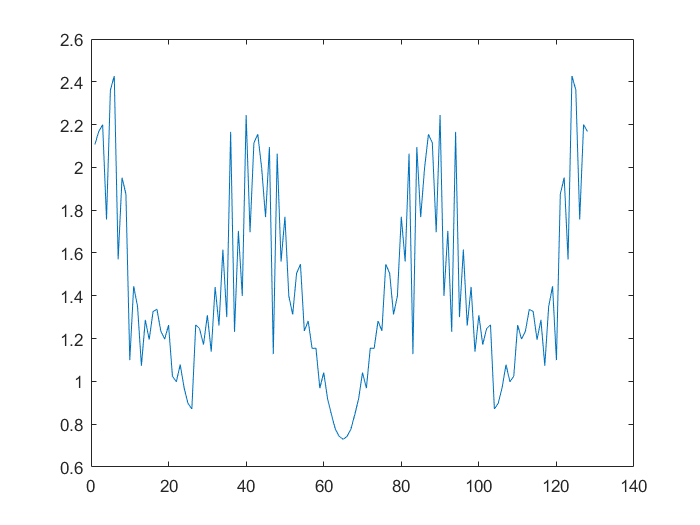
\includegraphics[scale=0.45]{../EJ1/periodogramaNP}
\caption{Estimaci\'on de la densidad espectral de potencia de $X(n)$ a partir de la promediaci\'on de periodogramas.}
\label{perio}
\end{figure}

Se observa que las densidades resultantes son bastante similares, con pequeñas diferencias. De esto se desprende que es posible estimar la densidad espectral con grupos de muestras más pequeños, promediando las densidades intermedias. Es decir, sin tomar demasiados datos se logra cometer muy poco error con el estimador promedio.

%%%%%%%%%%%%%%%%%%%%%%%%%%%%%
\newpage
\section*{Ejercicio 2}
Para el segundo ejercicio se pidió calcular Smoothing filters óptimos.
Para ello, se utilizó la ecuacion 7.83.b del Shanmugan con una pequeña modificación dado que los Smoothing filters tienen respuesta impulsiva no causal.
En primer lugar se define nuestra señal como X(n) = S(n) + v(n), donde S(n) es la señal de audio original y v(n) es ruido blanco gaussiano de media nula y se eligió una varia. Se estimaron las autocorrelaciones de X y de S utilizando la ecuación 9.6 del libro ``Random Signals'', K. Sam Shanmugan:
$$R_{xx}(k) = \frac{1}{N - k} \sum_{i=1}^{N-k-1}X(i)X(i+k)$$
 para luego obtener la respuesta impulsiva y finalmente realizar a convolución con la X, obteniendo el estimador a partir de la ecuación 7.74.

\begin{lstlisting}[language=Matlab, caption=Ejercicio2.m]
clear;
clc;
%leemos archivo (debe ser mono)
file = 'whereIam8Khz.wav';
info = audioinfo(file);
[data,Fs] = audioread(file);
t = 0:seconds(1/Fs):seconds(info.Duration);
S = compand(data,255,max(data),'mu/compressor'); % esta es la senal
Muestras = Fs*20e-3; %160 si fs 8Khz %fs*20ms = Muestras
Ventanas = cast(floor(length(S)/Muestras),'uint64'); 
S = S(1:Ventanas*Muestras); %Recortamos la senal en funcion de la cantidad de ventanas
PotRuido = -30; % esta en dB
Noise = wgn(length(S),1,PotRuido);
X_tot = S + Noise;
% La variable size determina la longitud de la respuesta impulsiva
% La longitud seria de 2*size+1
size = 10;
m = -size:size;
shat = double.empty; %en esta variable guardaremos el S estimada
for l=0:Ventanas-1
    td = (1+l*Muestras):(Muestras+l*Muestras);
    Act_X = X_tot(td);    
    Act_S = S(td);
    Rxx = get_Rxx(Act_X, Muestras,2*size+1);
    Rss = get_Rxx(Act_S, Muestras,size+1);
    RssMat = 1:size*2+1;
    for i=1:size*2+1
        index =  abs(size+1-i)+1;
        RssMat(i) = Rss( index );
    end
    R = toeplitz(Rxx);
    h = R\RssMat';
    Shift_H = circshift(h,size); % hacemos un shifteo a la 
    % respuesta impulsiva dado que no es causal
    estimacion = conv(Act_X,Shift_H,'same');        
    shat = [shat estimacion'];
end
subplot(3,1,1);
plot(t(1:length(S)),S)
title('Original')
subplot(3,1,2);
plot(t(1:length(X_tot)),X_tot)
title('Con ruido')
subplot(3,1,3);
plot(t(1:length(shat)),shat)
title('Estimacion')
player = audioplayer(shat, Fs);
play(player);
%para parar el audio stop(player);
\end{lstlisting}

\begin{lstlisting}[language=Matlab, caption=getRxx.m]
function [ Rxx ] = getRxx(x,N,k)
%Esta funcion es para obtener el estimador de la autocorrelacion de X
%Esta en la pagina 567 del Shanmugan
% x es el vector con las muestras
% N es la cantidad de muestras
% k es hasta donde calcular Rxx
Rxx = double.empty ;
for j = 0:k-1
    sumatoria = 0;
    for i = 0:N-j-1
        sumatoria = sumatoria + x(i+j+1)*x(i+1); % calculo la sumatoria
    end
    Rxx(j+1) = (1/(N-j))*sumatoria; % los sumo y divido por el k correspondiente
end
end

\end{lstlisting}


\begin{figure}[H] %!ht
\centering
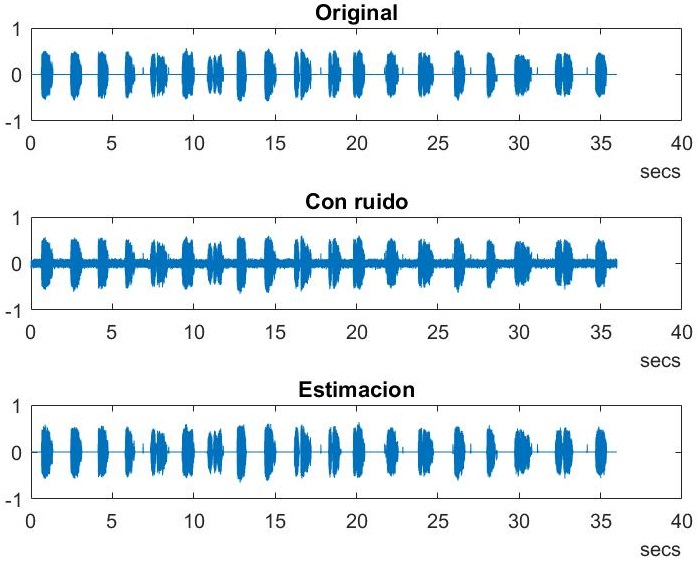
\includegraphics[scale=0.7]{../EJ2/EJ2.jpg}
\caption{Estimación de la señal de prueba 'whereIam8Khz.wav'}
\label{EstimacionWhereIam}
\end{figure}

Se puede ver en el primer gráfico de la figura la señal original, en la segunda se puede observar como se distorsiona la señal por efecto del ruido y en la tercera la estimación dada por el filtro obtenido. Se nota una gran similitud con la señal original.



\subsubsection{Conclusiones}
Durante la realizacion de este trabajo se pudo verificar el correcto funcionamiento de los "smoothing filters". Se logró a traves de la implementacion de uno obtener una estimacion muy similar a la señal original.


\end{document}
